\chapter{Technologies-and-Methodologies}
\label{chap:technologies_and_methodologies}

This chapter describes the technologies used to support SafeVision's processing of both still images and video, including frontend interaction, backend processing, machine learning integration, and deployment infrastructure.

\section{Frontend Technologies}

The frontend of the SafeVision system was developed as a web-based application using modern JavaScript technologies. The technology stack was selected to support interactive processing of both still images and video, efficient user workflows, and privacy-aware handling of sensitive data.

\methodheading{Core Frontend Framework}

The frontend is implemented using React in combination with TypeScript. React was chosen due to its component-based architecture \cite{react_components}, which enables modular and reusable user interface development by decomposing complex interfaces into smaller components. In addition, React’s rendering model is based on the concept of a virtual DOM \cite{react_virtual_dom}, which allows efficient updates by re-rendering only the parts of the interface that change \cite{virtual_dom_overview}, thereby improving performance in dynamic applications. This combination is particularly suitable for SafeVision, where interactive visualization of still images and video frames, together with real-time updates of detection results, requires efficient rendering and modular UI components.

TypeScript was used to introduce static typing to the codebase, providing improved reliability by catching errors during development \cite{typescript_benefits} and enhancing maintainability through clearer interfaces between components. This is particularly beneficial in larger systems where multiple modules interact and evolve over time.

To streamline the development workflow, Vite was selected as the build tool and development server \cite{vite}. Vite provides fast hot module replacement and efficient production builds through native ES module support, enabling rapid iteration during development and improved runtime performance in the deployed application.

In addition, React’s extensive ecosystem provides access to a wide range of third-party libraries and tools, supporting faster development and easier integration of additional functionality.

\methodheading{User Interface and Styling}

The user interface was implemented using modern CSS techniques, with Tailwind CSS as the primary styling framework. Tailwind CSS is a utility-first framework \cite{tailwind_css} that enables developers to construct user interfaces directly within component markup, reducing the need for separate CSS files and improving development efficiency. This approach allows rapid iteration and fine-grained control over styling \cite{utility_first_css}, which is particularly useful in interactive applications.

As illustrated in Figure~\ref{fig:tailwind_comparison}, Tailwind CSS differs from traditional CSS by applying utility classes directly within the markup rather than relying on separate style sheets. This reduces context switching during development and enables faster iteration when modifying user interface components. This is particularly beneficial in SafeVision, where interactive editing of detected regions requires rapid UI updates and precise control over visual elements. This approach also promotes consistency in styling by encouraging the reuse of predefined utility classes, reducing variability in design across components.

\begin{figure}[H]
\centering
\begin{minipage}{0.45\textwidth}
\textbf{Traditional CSS}
\begin{lstlisting}[language=HTML]
<button class="btn-primary">Continue</button>
\end{lstlisting}

\begin{lstlisting}
.btn-primary {
  height: 40px;
  padding: 0 16px;
  border-radius: 12px;
  font-size: 14px;
  font-weight: 500;
  border: 1px solid #374151;
  background-color: #111827;
  color: #f9fafb;
}
\end{lstlisting}
\end{minipage}
\hfill
\begin{minipage}{0.45\textwidth}
\textbf{Tailwind CSS}
\begin{lstlisting}[language=HTML]
<button class="h-10 px-4 rounded-xl text-sm 
font-medium border border-gray-700 
bg-neutral-900 text-gray-100 
hover:border-gray-400 transition">
  Continue
</button>
\end{lstlisting}
\end{minipage}

\caption{Comparison between traditional CSS and Tailwind CSS. The traditional approach separates styling into external stylesheets, while Tailwind CSS applies utility classes directly in the markup, enabling faster iteration and more localized styling.}
\label{fig:tailwind_comparison}
\end{figure}

The frontend was designed to support a human-in-the-loop workflow, where automated detection is combined with manual user control. Interactive interfaces play a key role in such systems \cite{human_in_loop_ai}, as they allow users to review and refine automated outputs. The interface therefore includes components for image visualization, control panels, and editing tools, enabling users to inspect detected regions and apply redaction methods while maintaining clarity and responsiveness, which are central usability principles \cite{usability_nielsen}.

The interface supports advanced user interactions such as zooming, panning, and direct manipulation of bounding boxes. These interactions are implemented using custom event handling and contribute to a more precise and efficient editing workflow, particularly when working with high-resolution images.

In addition to styling and layout, efficient rendering of visual elements is essential for interactive applications.

\methodheading{Canvas-Based Rendering}

The frontend utilizes HTML5 canvas-based rendering to support interactive visualization and manipulation of both still images and video frames. Canvas rendering enables efficient drawing and updating of graphical elements such as bounding boxes and overlays, which is essential for real-time interaction with detection results. Compared to standard DOM-based rendering, the canvas approach provides better performance for frequent graphical updates and fine-grained control over rendering behavior. This approach allows users to modify, resize, and reposition detected regions directly within the interface, supporting the human-in-the-loop workflow of the system. The same rendering approach is used to display overlays for video detections on individual frames, allowing consistent interaction patterns across image and video workflows.

\methodheading{State Management}

State management is handled using React’s built-in hooks and context mechanisms, enabling shared application state across components. Centralized state handling ensures consistent synchronization of updates throughout the interface \cite{react_state_management}. This is particularly important in SafeVision, where user interactions such as modifying bounding boxes, filtering detection results, or adjusting redaction settings require immediate and consistent updates across multiple UI components.

\begin{figure}[H]
\centering
\begin{tikzpicture}[
    node distance=1.6cm,
    every node/.style={font=\small},
    state/.style={
        rectangle, 
        rounded corners, 
        draw=black, 
        minimum width=3.2cm, 
        minimum height=0.8cm, 
        align=center
    },
    arrow/.style={->, thick}
]

% Nodes
\node[state] (upload) {User Upload};
\node[state, below of=upload] (image) {Frontend State: Visual Media};
\node[state, below of=image] (api) {API Call to Backend};
\node[state, below of=api] (results) {Detection Results};
\node[state, below of=results] (boxes) {Frontend State:\\ Bounding Boxes};

\node[state, below left=1.2cm and 1.8cm of boxes] (edit) {User Edits};
\node[state, below right=1.2cm and 1.8cm of boxes] (auto) {Auto Results};

\node[state, below of=boxes, yshift=-2cm] (updated) {Updated State};
\node[state, below of=updated] (redact) {Redaction Applied};
\node[state, below of=redact] (output) {Final Output};

% Arrows (main flow)
\draw[arrow] (upload) -- (image);
\draw[arrow] (image) -- (api);
\draw[arrow] (api) -- (results);
\draw[arrow] (results) -- (boxes);

% Branches
\draw[arrow] (boxes) -- (edit);
\draw[arrow] (boxes) -- (auto);

% Merge
\draw[arrow] (edit) -- (updated);
\draw[arrow] (auto) -- (updated);

% Final flow
\draw[arrow] (updated) -- (redact);
\draw[arrow] (redact) -- (output);

\end{tikzpicture}

\caption{State management and data flow in the frontend application. The figure illustrates how visual media data and detection results are stored, updated, and transformed throughout the user workflow, including backend communication and user-driven modifications.}
\label{fig:state-management-flow}

\end{figure}

\methodheading{Client-Side Storage and Privacy Considerations}

To support privacy-by-design principles, the SafeVision frontend utilizes a combination of client-side storage mechanisms, primarily localStorage and IndexedDB. These technologies enable persistent storage of application data directly within the user’s browser, reducing the need to transmit sensitive information to external servers and aligning with data minimization principles defined in GDPR \cite{gdpr_reference}.

LocalStorage is used for lightweight configuration data, such as user preferences and interface settings. This includes information such as theme selection, UI layout configurations, and user consent status. These data elements are small in size and require simple key-value storage, making localStorage a suitable and efficient solution.

In contrast, IndexedDB is used for storing larger and more complex data structures, such as image annotations and video processing results. IndexedDB provides an asynchronous and structured storage model, allowing efficient handling of larger datasets without blocking the main application thread. This is particularly important in SafeVision, where annotation data may include multiple bounding boxes and metadata associated with high-resolution images and video frames.

Figure~\ref{fig:indexeddb_storage} illustrates the structure of client-side storage used in the application. The system maintains multiple logical databases and object stores to separate concerns such as image annotations and video-related data, improving maintainability and scalability.

\begin{figure}[H]
\centering
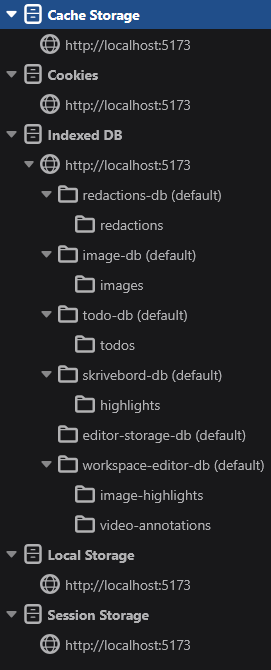
\includegraphics[height=0.4\textheight]{figures/images/chapter-7/storage-solution.png}
\caption{Overview of client-side storage in the application using IndexedDB.}
\label{fig:indexeddb_storage}
\end{figure}

As shown in Table~\ref{tab:storage_overview}, the storage design separates lightweight configuration data from larger annotation data. This distinction ensures efficient use of browser storage mechanisms while maintaining responsiveness and scalability in the application.

\begin{table}[H]
\centering
\begin{tabular}{|p{4cm}|p{3cm}|p{7cm}|}
\hline
\textbf{Storage Key / Store} & \textbf{Storage Type} & \textbf{Purpose} \\
\hline
workspace:consent:gdpr:v1 & localStorage & Stores whether the user has accepted the terms and conditions, ensuring compliance with GDPR requirements. \\
\hline
workspace:user-preferences:v1 & localStorage & Persists user interface preferences such as theme, highlight styles, and interaction settings across sessions. \\
\hline
workspace:sidebar:width & localStorage & Stores the current width of the sidebar to maintain a consistent layout between sessions. \\
\hline
workspace:patch-notes:seen-version & localStorage & Tracks which version of patch notes the user has already viewed to avoid repeated notifications. \\
\hline
image-highlights & IndexedDB & Stores bounding box annotations for images, including manually adjusted and automatically detected regions. \\
\hline
video-annotations & IndexedDB & Stores structured detection results for video frames, enabling persistence of annotations across sessions. \\
\hline
\end{tabular}
\caption{Overview of client-side storage keys and their purposes in the SafeVision frontend.}
\label{tab:storage_overview}
\end{table}

\methodheading{API Communication}

Communication between the frontend and backend is performed through HTTP-based API requests following REST principles. RESTful architectures \cite{rest_fielding} provide a standardized and scalable approach to communication between distributed systems, enabling a clear separation between client and server responsibilities. A structured service layer is used to manage these interactions, improving maintainability and the separation of concerns.

Together, these technologies provide a flexible and efficient foundation for developing an interactive, responsive, and privacy-aware frontend application.

\section{Backend Technologies and Languages}

The backend system was developed in Python, which was used for the computer vision components, the machine learning pipeline, and the FastAPI-based communication layer between the frontend and backend. This choice provided a consistent technology stack across the backend while also taking advantage of Python’s extensive library ecosystem for machine learning, image processing,
and frame-based video processing.

Machine learning components in the image redaction system follow a structured development pipeline consisting of data preparation, model training, and deployment. This process is applied to all detection models used in the system, including face detection, text detection, and QR/barcode detection.


\methodheading{FastAPI Application and API Structure}

The backend of SafeVision was implemented using FastAPI as the main application
framework. FastAPI was selected because it provides a lightweight and efficient
way to define REST-based APIs, while also supporting asynchronous request
handling. This made it well suited for a system that performs visual media processing and machine learning inference, where responsiveness and scalability are
important.

FastAPI also provides automatic request validation and clear endpoint
definitions, which simplified the implementation of the backend API and improved
maintainability during development.

Support for asynchronous execution was another important factor. Since detection
tasks may involve multiple independent models, the backend was designed to
support concurrent processing where possible. This contributes to better
responsiveness and improves the system’s ability to handle computationally
intensive tasks efficiently.


\methodheading{Backend Processing Utilities}

In addition to the FastAPI application layer, the backend relies on a set of
processing utilities that support image decoding, preprocessing, concurrent
execution, output normalization, and temporary file management. These utilities
were selected to make the backend pipeline more reusable and to reduce repeated
logic across detection and redaction endpoints.

For image handling, the backend uses OpenCV and NumPy to decode uploaded image
files into array representations suitable for inference and image processing.
This provides efficient low-level support for reading, transforming, and
encoding image data in the detection and redaction pipeline.

Model-specific preprocessing is handled through shared utility functions that
apply scaling, adaptive scaling, and optional preprocessing before inference.
This was important because the integrated detection models have different input
characteristics, and a shared preprocessing layer made it easier to support
multiple models without duplicating preparation logic across endpoints.

To improve responsiveness, the backend uses Python's \texttt{asyncio} utilities
to execute independent detection tasks concurrently where possible. This is
particularly relevant when multiple detectors are applied to the same image, as
it reduces waiting time compared with strictly sequential execution. At the same
time, synchronization mechanisms are used where necessary to avoid unsafe
concurrent access to shared processing resources in the redaction pipeline.

Another important utility layer concerns output normalization and validation.
Since the integrated models produce results in different formats, shared
processing logic is used to convert them into a unified representation before
they are returned through the API. This includes validation and adjustment of
bounding box coordinates to ensure that downstream components receive
well-formed results.

For video processing, the backend extends the same utility-based approach to frame-based media handling. OpenCV is used to open uploaded video files, read frames sequentially, access video properties such as frame rate and frame dimensions, and write temporary processed video output. This allows videos to be handled as sequences of image frames, while still relying on the same low-level image representation used by the rest of the backend.

The backend also uses FFmpeg as a final video-output utility. While OpenCV is
practical for writing processed frames during computation, FFmpeg is used
through the helper function \texttt{remux\_to\_h264\_aac(...)} to finalize the
processed video output and improve playback compatibility in browser and
media-player environments.

Because video processing involves larger files and intermediate outputs, the backend uses temporary file and directory handling based on Python’s standard file-management utilities. Uploaded videos, temporary processed files, and final outputs are isolated in request-specific working directories and cleaned up after detection or redaction has completed.

Table~\ref{tab:backend_processing_utilities} summarizes the main backend
processing utilities and their technical roles in the system.

\begin{table}[H]
\centering
\renewcommand{\arraystretch}{1.5}
\begin{tabular}{p{3.2cm} p{3.5cm} p{7cm}}
\toprule
\textbf{Utility area} & \textbf{Technology} & \textbf{Purpose} \\
\midrule
Image and video decoding and processing & \texttt{OpenCV}, \texttt{NumPy} & Decode uploaded image files and video frames, convert visual data into array representations, and support low-level processing in detection and redaction workflows. \\

Video output finalization & \texttt{FFmpeg} & Finalize processed video files through \texttt{remux\_to\_h264\_aac(...)} to improve playback compatibility across clients. \\

Preprocessing support & Shared preprocessing utilities & Apply scaling, adaptive resizing, and optional preprocessing before inference for different detection models. \\

Concurrent execution & Python \texttt{asyncio} & Run independent detection tasks concurrently to improve backend responsiveness. \\

Synchronization & Python \texttt{asyncio.Lock} & Prevent unsafe concurrent execution in shared parts of the redaction pipeline. \\

Output normalization & Shared normalization logic & Convert heterogeneous model outputs into a unified response format for frontend integration and downstream processing. \\

Temporary workspace handling & \texttt{tempfile}, \texttt{pathlib}, \texttt{shutil} & Manage request-specific temporary files and directories for video upload, intermediate processing, output generation, and cleanup. \\
\bottomrule
\end{tabular}
\caption{Overview of backend processing utilities used in the SafeVision backend.}
\label{tab:backend_processing_utilities}
\end{table}



\section{Machine Learning Technologies and Development Environment}

SafeVision relies on a separate machine learning development environment for
dataset preparation, model training, and evaluation of custom models. This
environment was maintained in a dedicated repository, while the deployed
SafeVision application was implemented in a separate repository focused on
inference, redaction, API handling, and frontend interaction.

\begin{figure}[H]
\centering
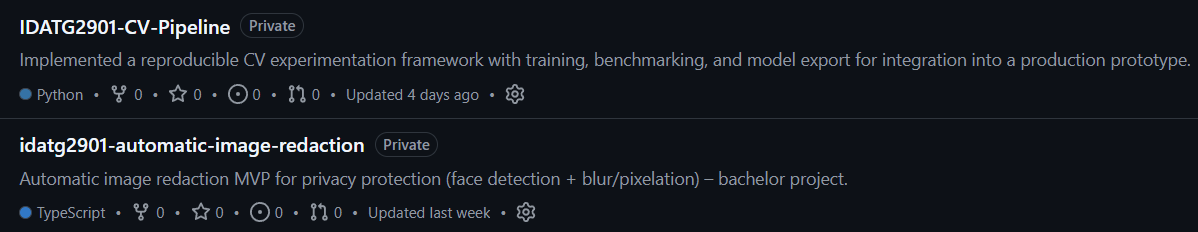
\includegraphics[width=1.0\textwidth]{figures/images/chapter-8/cv_repos.png}
\caption{Separation between the machine learning development repository and the
SafeVision application repository. The development repository was used for
dataset preparation, training, and evaluation, while the SafeVision repository
contains the deployed inference and redaction system.}
\label{fig:cv_repos}
\end{figure}

This separation was motivated not only by workflow considerations, but also by
technical differences between the two environments. Model development required
heavier machine learning dependencies, dataset-processing scripts, training
utilities, and evaluation workflows that were not needed in the deployed
application. Keeping these concerns separate reduced dependency conflicts and
made it easier to manage different library versions, requirements files, and
virtual environments for training and deployment.

The machine learning environment was used for the development of the custom
YOLOX-based object detection models for barcode and license plate detection, as
well as the text analysis components used for selective text redaction. In the case 
of text processing, this included a fine-tuned named entity recognition model adapted 
for Norwegian and English text. These components required a different development
setup from the production backend, where the main goal was stable inference rather
than iterative experimentation.

\begin{figure}[H]
\centering
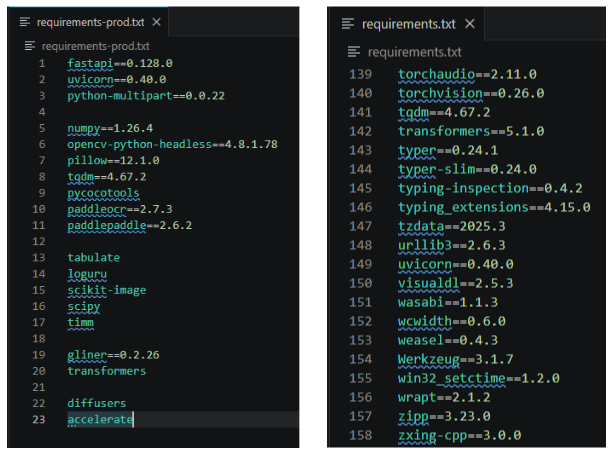
\includegraphics[width=0.7\textwidth]{figures/images/chapter-7/requirements.png}
\caption{Excerpts from \texttt{requirements.txt} and \texttt{requirements-prod.txt}, 
showing the difference in dependency set size.} 
\label{fig:requirements_comparison}
\end{figure}

The specific training, preprocessing, and integration steps are described in
Chapter~\ref{chap:implementation_details}. The present section instead focuses
on the technological and environmental choices that supported machine learning
development across the two repositories.

\section{Deployment and Infrastructure}

The project relied on a small set of deployment and infrastructure technologies
to support delivery, automation, and collaboration. Docker was used for
containerization, GitHub Actions for CI/CD automation, Google Cloud for hosting
and deployment, and GitHub for version control and team collaboration.

\begin{table}[H]
\centering
\begin{tabular}{p{3.2cm} p{4cm} p{6.5cm}}
\toprule
\textbf{Technology} & \textbf{Role} & \textbf{Purpose in the project} \\
\midrule
Docker & Containerization & Package the backend and its dependencies into a consistent runtime environment. \\

GitHub Actions & CI/CD automation & Automate validation, build, and deployment workflows. \\

Google Cloud & Cloud platform & Host and deploy the backend and frontend application components. \\

GitHub & Version control and collaboration & Support branch-based development, code sharing, and team coordination. \\
\bottomrule
\end{tabular}
\caption{Deployment and infrastructure technologies used in the project.}
\label{tab:deployment_infrastructure_tech}
\end{table}

Docker was used to package the backend application and its dependencies into a
consistent runtime environment. This reduced environment-specific issues and
simplified deployment across development and production stages.

GitHub was used for version control, code sharing, and collaboration throughout
the project. This supported branch-based development, change tracking, and team
coordination. In addition, GitHub Actions was used to implement CI/CD. The CI
workflow was used to validate changes through automated checks, while the CD
workflow was used to build and deploy updated application artifacts.

Google Cloud was used as the deployment platform for the SafeVision system. It
provided the cloud environment used to host the deployed application
components.
